\documentclass[aps,twocolumn,preprintnumbers,amsmath,amssymb,nofootinbib,superscriptaddress,notitlepage]{revtex4-1}
%
%=============================================================================
%\usepackage[margin=1.in]{geometry}
\usepackage{slashed}
\usepackage{amssymb}
\usepackage{mathtools}
\usepackage{bbold}
\usepackage{amssymb,latexsym}
\usepackage{amsmath,amsbsy,bbm}
\usepackage{multirow}
\usepackage[vcentermath]{youngtab}
\usepackage{nicefrac}
\usepackage[perpage]{footmisc}
\usepackage{wrapfig,lipsum,booktabs}
\usepackage{caption}
\usepackage{subcaption}
\usepackage{cjhebrew}
\usepackage{tikz,pgfplots}
\usetikzlibrary {graphs}

%\usepackage{physics}
\usepackage{floatrow} 
%\newfloatcommand{capbtabbox}{table}[][\FBwidth]
%=============================================================================
\newfloatcommand{capbtabbox}{table}[][0.45\textwidth]
%\DefineFNsymbols*{lamportnostar}[math]{\dagger\ddagger\S\P\|{\dagger\dagger}{\ddagger\ddagger}}
%\setfnsymbol{lamportnostar}
%\renewcommand\thefootnote{\fnsymbol{footnote}}
%=============================================================================
\usepackage{nicematrix}
\NiceMatrixOptions{
code-for-first-row = \color{blue} ,
code-for-last-row = \color{blue} ,
code-for-first-col = \color{blue} ,
code-for-last-col = \color{blue}
}

\newcommand{\es}{1\text{\scriptsize s}}
\newcommand{\zs}{2\text{\scriptsize s}}
\newcommand*{\mprime}{^{\prime}\mkern-1.2mu}
\newcommand{\largescale}{\ensuremath{\Lambda_\text{Hi}}}
\newcommand{\lc}{\ensuremath{\Lambda_c}}
\newcommand{\fm}{\ensuremath{\,\text{fm}^{-1}}}
\newcommand{\abb}{\mbox{\ensuremath{A\oplus 1}}}
\newcommand{\red}[1]{\textcolor{red}{#1}} 
\newcommand{\green}[1]{\textcolor{green}{#1}} 
\newcommand{\blue}[1]{\textcolor{blue}{#1}} 
\newcommand{\lec}{C^\Lambda}
\newcommand{\led}{D^\Lambda}
\newcommand{\ddrei}[1]{\delta_{\tiny \Lambda}^{(3)}\!\big(#1\big)}
\newcommand{\wrt}{\textit{w.r.t.}~}
\newcommand{\etc}{\textit{etc.}~}
\newcommand{\eg}{\textit{e.g.}~}
\newcommand{\ie}{\textit{i.e.}~}
\newcommand{\viz}{\textit{viz.}~}
\newcommand{\eftnopi}{\mbox{EFT$(\not \! \pi)$}}
\newcommand{\ve}[1]{\ensuremath{\boldsymbol{#1}}}
\newcommand{\rms}[1]{\ensuremath{\langle r(#1)\rangle}}
\newcommand{\ls}{\ve{L}\cdot\ve{S}}
\newcommand{\be}{\begin{equation}}
\newcommand{\ee}{\end{equation}}
\newcommand{\bra}{\big\langle}
\newcommand{\ket}{\big\rangle}
\newcommand{\hl}{\big\vert}
\newcommand{\vcl}[1]{\ensuremath{\bar{\boldsymbol{r}}_\text{\tiny #1}}}
\newcommand{\vsp}[1]{\ensuremath{\boldsymbol{r}}_\text{\tiny #1}}
\newcommand{\la}{\label}
\newcommand{\Pe}{\text{\cjRL{p|}}}
\newcommand{\figref}[1]{fig.~\ref{#1}}
\newcommand{\tabref}[1]{table~\ref{#1}}
\newcommand{\secref}[1]{sec.~\ref{#1}}
\newcommand{\ccite}[1]{Ref.~\cite{#1}}
\newcommand{\dbra}[1] {\left\langle~#1~\right|}
\newcommand{\dket}[1] {\left|~#1~\right\rangle}
\newcommand{\bet}[1] {\left|#1\right|}
\newcommand{\overlap}[2] {\left\langle\,#1\,\left|\,#2\,\right.\right\rangle}
\newcommand{\me}[3] {\left\langle\,#1\,\left|\left.\,#2\,\right|\,#3\,\right.\right\rangle}
\newcommand{\redme}[3] {\left\langle\,#1\,\middle|\right|\,#2\,\left|\middle|\,#3\,\right\rangle}

\definecolor{blue}{HTML}{4169E1}
\definecolor{red}{HTML}{DC143C}
\definecolor{green}{HTML}{2E8B57}
\definecolor{mandarin}{HTML}{FF9933}

\newcommand{\MPV}[1]{\textcolor{purple}{#1}}
\newcommand{\LC}[1]{\textcolor{mandarin}{#1}}
\newcommand{\JK}[1]{\textcolor{green}{#1}}
\newcommand{\note}[1]{\textbf{\textcolor{gray}{#1}}}

\DeclareMathOperator{\sign}{sign}

%=============================================================================
\usepackage[normalem]{ulem}

\DefineFNsymbols*{lamportnostar}[math]{\dagger\ddagger\S\P\|{\dagger\dagger}{\ddagger\ddagger}}
\setfnsymbol{lamportnostar}
\renewcommand\thefootnote{\fnsymbol{footnote}}
\let\endtitlepage\relax

\begin{document}

\title{Universal aspects of the multi-channel 4-body scattering system}
\author{Sourav Mondal}
\author{Rakshanda Goswami}
\author{Udit Raha}
\address{Department of Physics, Indian Institute of Technology Guwahati, Guwahati 781039, India}
\author{Johannes Kirscher}
\address{Department of Physics, SRM University - AP, Amaravati 522502, Andhra Pradesh, India}
\date{\today}

\begin{abstract}
We investigate the scattering system of 4 equal-mass quantum particles at energies
which allow for open rearrangement channels with an interaction that approaches the
unitary limit sustaining a 2-body bound state at threshold.

As a benchmark, we obtain the universal ratio of the elastic dimer-dimer scattering length
to the scattering length between the two fermions which constitute each dimer.
Subsequently, we extend the analysis to a 4-component-fermion system in which a new scale
enters in form of a bound trimer.
We commence the study with spin- and fermion-species-independent contact interactions
between two and three particles with single 2- and 3-body bound states of non-zero energy.
We find a hierarchy of dimer-dimer scattering lengths which follows from the different
couplings of the three degenerate dimer-dimer channels with the two trimer-fermion channels.
Counter-intuitively, we find this hierarchy reversed in the unitary limit when dimer-dimer,
dimer-fermion-fermion, and 4-fermion thresholds merge.

Specifically, we obtain ratios of 3-1 and 2-2 scattering lengths as functions of the 3-body
scale as unitarity is approached from a dimer resembling the deuteron. All observables are
subjected to a renormalization-group analysis in form of a regulator-cutoff variation.
Aside from a cusp close to the 3-1 threshold, we do not find signatures of resonant behaviour. 
\end{abstract}

\maketitle

\section{Introduction}
The four-fermion quantum scattering problem exhibits most features any interaction theory
which aspires to be useful for the description of low-energy nuclear and atomic few-body
must include. A lot has been learned, in particular, about the nuclear force from decades of
studies aiming for a theoretical description consistent with experimental data for resonances,
coupled angular-momentum and rearrangement channels, and relatively closely spaced thresholds.
While these endeavours aimed for a comprehensive description of low- and high-energy observables,
an attempt to expand the nuclear interaction commences with a leading-order which allows for
relatively large uncertainties which are reduced by considering higher-orders systematically.
The arguably most significant success of the adaptation of this framework of an effective field
theory (EFT) to bound-state observables of few-body systems has been the identification of certain
properties which are universal to atoms, nuclei, hadrons, clusters, and other quantum particles
whose short-distance structures differ but which exhibit a notable separation of scales between
their interaction ranges ($r$) and typical 2-body scales ($a$), \eg, the range of the nuclear force being relatively
small compared to the spatial extend of the deuteron.

In the theoretical limit, $\vert r/a\vert\to 0$, the scale-free 2-body system is uncorrelated
with observables of systems involving more than two particles which evolve subject to the
interaction underlying this limit. For instance, a van der Waals inter-atomic potential and
a zero-range contact interaction which both yield $\vert r/a\vert= 0$ will evoke identical few-body
observables: the Efimov spectrum in cases which allow for a totally symmetric spatial wave function,
and the amount of attenuation of the effective interaction between two dimers\footnote{We adopt the dimer-trimer-tetramer
notion for bound states of two, three, and four particles.} compared with the force which
binds the dimers. The latter was quantified in terms of the ration of the pertinent scattering lengths,
$a_{dd}=0.6\,a$, for 2-component fermions (2CF) which by themselves cannot realize the spatial symmetry required
for Efimov spectra. These two examples of universal behaviour represent bound-state and scattering observables
emerging in bosonic and fermionic systems.

In this article, we expand on the second phenomenon: scattering observables which are found in all
systems which realize, or are close to the limit $\vert r/a\vert\to 0$, and their dependence on the
particle statistics. In particular, we analyse features of the 4-body scattering system which result
from bose statistics and are thus relevant for the prominent $J^\pi=0^+$ helium-4/$\alpha$ channel. Without reference
to a specific type of fermion, we characterize the problem as follows: What kind of 4-body scattering matrix follows
from a spin- and species-independent\footnote{We avoid the nuclear term {\it isospin} and thus refer to neutrons
and protons in their respective spin up/down states as {\it species} with labels 1,2 in the 2CF case, and 1,2,3,4
for 4CF, such that, \eg, proton-spin-up $\hat{=}1$.} 2-body interaction which approaches the
{\it unitary} limit $\vert r/a\vert\to 0$ for any pair of 4-component (4CF), equimassive fermions?

Firstly, we will specify the structure of interaction we chose to realize the unitary limit including the method
to assess the sensitivity of our finding with respect to variations of this choice. Secondly, we define the
scattering problem approximated by five asymptotic two-fragment channels and its variational solution. The latter
is presented separately for the uncoupled, fermionic case and the coupled scenario in subsequent sections followed by
an out-looking conclusion.

 
\section{Interaction theory}

The minimal theory from which the wealth of nuclear, atomic, and all other approximately unitary systems can be developed
systematically uses a Hamiltonian of the form

\be\la{eq.ham}
H^{(0)}
=
\sum_iT_1(\vsp{i},m)
+
\sum_{\lbrace i,j\rbrace}V_2(\vsp{ij},\lambda)
+
\sum_{\lbrace i,j,k\rbrace}V_3(\vsp{ij},\vsp{ik},\lambda)
\ee 

comprising a 1-particle kinetic energy and 2- and 3-particle potentials
depending on single-particle and one or two relative coordinates, respectively.
$\lambda$ differentiates between different potential forms which all yield
a two body system at/close-to unitarity.
The appearance of a 3-body potential is due to our choice for the 2-body
potential which reduces to a zero-range contact interaction and thus is characterized
by a single strength that is tuned to the unitarity condition $\vert a\vert\approx\infty$.
Hence, the 3-body scale needs to enter differently in form of a 3-particle operator.
The superscript identifies the hamiltonian as the leading order (LO) of an EFT expansion,
and we limit the study to particles with equal masses $m$.
For practical reasons related to the numerical method (see \secref{sec.scatprob}), we limit
the renormalization-group (RG) transformation to those interactions which are represented by

\be\la{eq.2pot}
V_2 
= 
c(\lambda) \,
e^{-\lambda\,(\ve{r}_i-\ve{r}_j)^2}
\;\;
,
\qquad
\ee

and

\be\la{eq.3pot}
V_3 = 
d(\lambda)\,  
e^{-\lambda\,\left[ (\ve{r}_i-\ve{r}_j)^2 + (\ve{r}_i-\ve{r}_k)^2\right]}
\qquad
.
\ee

The RG parameter is thus identical to a cutoff, each value of which corresponding to an interaction
which, by definition, must furnish a scattering length $a$ much larger than the interaction range $r\sim\lambda^{-1}$.
Instead of renormalizing the low-energy constant (LEC) $c(\lambda)$ to such an $a$, we constrain it by
a sequence of 2-body binding energies $B(2)\to0$ in order to take the limit to unitarity.

Here, in addition to the spatial location, we consider single-particle states occupying one of two or one out of four internal states,
\eg, the two spin orientations of a pure neutron system, or the four states of a nucleon: neutron/proton spin-up/down.
From the invariance of $H^{(0)}$ with respect to any transposition $i\leftrightarrow j$ and the anti-symmetry of the system's wave function
thereunder, physical matrix elements of $V_3$ vanish for states comprised solely of 2CF. Hence, such systems
do not form trimers. The formation of trimers, the non-vanishing $V_3$, the emergence of a unique 3-body scale, can be understood
as consequences of the continuous scale symmetry which characterizes the unitary 2-body system being broken and realized
discretely in the 3- and more-body sector of 4CF.
The existence of trimers and of four degenerate dimer states (see \secref{sec.scatprob})
defines five coupled channels for the 4CF 4-body system which we will describe in the next section.

Succinctly stated, the problem of identifying properties of an arbitrary $N$-fermion systems which exhibits an approximately
scale-free 2-body sector is encoded in the solution to

\be\la{eq.sgl}
H^{(0)}
\hat{\mathcal{A}}_N
\dket{\lbrace\vsp{i},\tau_i\rbrace}_n
=
E_n
\hat{\mathcal{A}}_N
\dket{\lbrace\vsp{i},\tau_i\rbrace}_n
\ee
with $\tau_i\in\lbrace1,\ldots,\text{nbr. of species}\rbrace$,
the anti-symmetrizer $\hat{\mathcal{A}}=\sum_{\mathcal{P}\,\in\,\mathcal{S}_N}\sign(\mathcal{P})\,\mathcal{P}$,
and a $H^{(0)}$ properly renormalized to the unitary 2-body system and a 3-body scale of choice. To access the bound-state
spectrum, the boundary condition

\be\la{eq.bcbs}
\lim_{\vert\vsp{ij}\vert\to\infty}
\underbrace{
\overlap{\lbrace\vsp{i}\rbrace}{\lbrace\vsp{i},\tau_i\rbrace}_n
}_{=:\Psi_n}
=
0
\ee
must be met $\forall i\neq j$ and $E_n<0$.

\section{The scattering problem}\la{sec.scatprob}

The scattering problem imposes boundary conditions pertinent to specific incoming
and outgoing states which are defined in the infinite past and future, respectively.
A complete set of these asymptotic states includes all partitions of the $N$ particles
into infinitely separated, bound fragments. However, if the interest is on reactions
between two fragments at energies which are relatively small compared with their lowest
separation energies, a 2-fragment approximation of the asymptotic wave function

\be\la{eq.2frag}
\Psi_n\to\phi^{(1)}\,\chi(\vsp{\text{rel}})\,\phi^{(2)}
\ee

suffices.

\subsection{Asymptotic states}
For an interaction which does not depended on the intrinsic state of a particle, \ie,
acts alike between all pairs of elements of a spin-isospin multiplet, a scattering
channel is defined solely by: total number of each particle species in the system (relevant
for obtaining the correct (anti)symmetrization), orbital-angular-momentum structure (consistent with
the order of the EFT expansion of the interaction), a fragmentation of the particles into bound clusters
(any selection of species to furnish a cluster which allows for a totally antisymmetric internal wave function
is legitimate. A discrimination between various (iso)spin coupling schemes only produces redundant channels). 

The zero-range, momentum-independent LO interaction supports only bound states with a totally symmetric spatial wave function.
Hence, component particles of the state cannot occupy identical fermionic states, and the asymptotic fragments are
to be taken from the following lists\footnote{Roman particle-species labels on the same object are understood, here, to
assume different values, only, \eg, $(i,j)$ can mean $(1,3)$ but never $(2,2)$.}.

\begin{align*}
(2\text{CF})~&:~\phi^{(1,2)}\in\lbrace i,(i, j):i,j\in\lbrace 1,2\rbrace\rbrace\\
(4\text{CF})~&:~\phi^{(1,2)}\in\lbrace i,(i, j),(i, j, k):i,j,k\in\lbrace 1,2,3,4\rbrace\rbrace\\
\end{align*}

Relative $S$-wave scattering between two fragments composed of 2CF is thus a single-channel problem:

\usetikzlibrary {graphs}
\tikz \graph [grow right sep, left anchor=east, right anchor=west] { a [as=$(ij)(ij)$] -> b [as=$(ij)(ij)$] };

The 4CF problem, in turn,


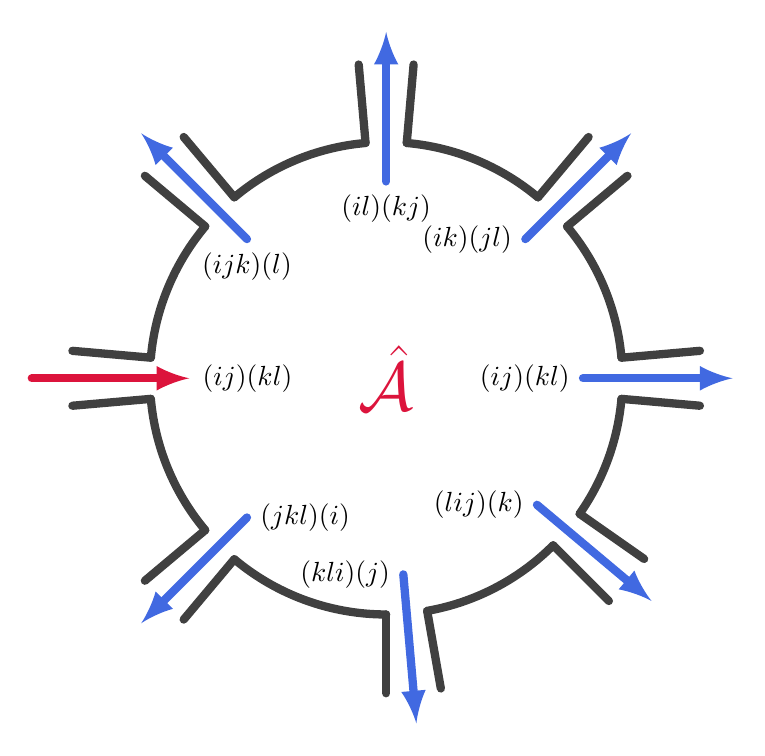
\begin{tikzpicture}[]
% Grid

%\foreach \i in {1,2,...,6}
%{
%\draw[lightgray!20] (0,0) circle(\i);
%}
%
%\foreach \i in {0,45,90,135,...,315}
%{
%\draw[lightgray!20] (0,0) -- (\i:7.2) node[pos=0.96,black,fill= white]{\i};
%}

% Puzzle

% circles
\begin{scope}[line width=3pt,cap=round, rounded corners=1pt,black!75]

\draw [domain=5:40] plot ({3*cos(\x)}, {3*sin(\x)});
\draw [domain=50:85] plot ({3*cos(\x)}, {3*sin(\x)});
\draw [domain=95:130] plot ({3*cos(\x)}, {3*sin(\x)});
\draw [domain=140:175] plot ({3*cos(\x)}, {3*sin(\x)});
\draw [domain=185:220] plot ({3*cos(\x)}, {3*sin(\x)});
\draw [domain=230:270] plot ({3*cos(\x)}, {3*sin(\x)});
\draw [domain=280:315] plot ({3*cos(\x)}, {3*sin(\x)});
\draw [domain=325:355] plot ({3*cos(\x)}, {3*sin(\x)});

\draw  (5:3) -- (5:4);
\draw  (-5:3) -- (-5:4);
\draw  (40:3) -- (40:4);
\draw  (50:3) -- (50:4);
\draw  (85:3) -- (85:4);
\draw  (95:3) -- (95:4);
\draw  (130:3) -- (130:4);
\draw  (140:3) -- (140:4);
\draw  (175:3) -- (175:4);
\draw  (185:3) -- (185:4);
\draw  (230:3) -- (230:4);
\draw  (220:3) -- (220:4);
\draw  (270:3) -- (270:4);
\draw  (280:3) -- (280:4);
\draw  (325:3) -- (325:4);
\draw  (315:3) -- (315:4);

\end{scope}

\draw[-latex,line width=3pt,cap=round, rounded corners=1pt,red] (180:4.5)--(180:2.5) node[right,black] {$(ij)(kl)$};

\draw[-latex,line width=3pt,cap=round, rounded corners=1pt,blue] (45:2.5)  node[left,black] {$(ik)(jl)$}--(45:4.4) ;
\draw[-latex,line width=3pt,cap=round, rounded corners=1pt,blue] (90:2.5)  node[below,black] {$(il)(kj)$} --(90:4.4) ;
\draw[-latex,line width=3pt,cap=round, rounded corners=1pt,blue] (135:2.5) node[below,black] {$(ijk)(l)$} --(135:4.4);
\draw[-latex,line width=3pt,cap=round, rounded corners=1pt,blue] (225:2.5) node[right,black] {$(jkl)(i)$} --(225:4.4);
\draw[-latex,line width=3pt,cap=round, rounded corners=1pt,blue] (275:2.5) node[left,black] {$(kli)(j)$} --(275:4.4);
\draw[-latex,line width=3pt,cap=round, rounded corners=1pt,blue] (320:2.5) node[left,black] {$(lij)(k)$} --(320:4.4);
\draw[-latex,line width=3pt,cap=round, rounded corners=1pt,blue] (0:2.5)   node[left,black] {$(ij)(kl)$} --(0:4.4)  ;
\draw[red,scale=2] (0,0) node {\Huge $\hat{\mathcal{A}}$};
\end{tikzpicture}


In more familiar terms, the 2CF dimer could be a spin-singlet isospin-triplet dineutron\footnote{The LO of the nuclear contact EFT without pions
binds two neutrons and lifts this degeneracy with the the spin-triplet state at higher orders.}. The four dimers composable from
4CF could be the deuteron, the spin-singlet neutron-proton, the di-neutron, and the di-proton. The two trimers would then
represent the triton/hydrogen-3 and the helion/helium-3. As any (iso)spin dependence, including electromagnetism,
enters at a higher order of the EFT expansion,
the binding energies off all dimers are degenerate and approach zero in the unitary limit. 
The two trimers are degenerate, too, but their energy is set by the specific choice of the 3-body scale.

There is only one set of four 2CF which allows for two bound fragments, namely, $(1212)$. For 4CF, we focus on that set which
finds all four particles in different internal states, \ie, $(1234)$, pertinent to the nuclear $0^+$ channel.
Hence, there is only one single elastic channel for 2CF, while the 4CF case allows for five rearrangement channels.
Both cases are covered with the following, general structure of the scattering wave function:

\begin{widetext}
\begin{eqnarray*}\la{eq.scatt}
\Psi_{c'}
&=
\hat{\mathcal{A}}
\left\lbrace
\sum_{\text{{\bf c}hannels}}
\phi^{(1)}_c\phi^{(2)}_c
\cdot
\left(
\delta_{c'c}u_0(kR)
+
a_{c'c}w_0^{(+)}(kR)
+
\sum_db_{c'd}\Phi_d
\right)
\right\rbrace
\\
&=
\left\lbrace
\begin{array}{ll}
\text{2CF}~:&\hat{\mathcal{A}}\left\lbrace\phi^{(1)}(\vsp{12})\phi^{(2)}(\vsp{34})\chi_0(R)\right\rbrace\\
\text{4CF}~:&\hat{\mathcal{A}}\left\lbrace\phi^{(1)}(\vsp{12})\phi^{(2)}(\vsp{34})\chi_0(R)\right\rbrace\\
\end{array}
\right.
\end{eqnarray*}
\end{widetext}


\section{Results (single-channel)}

\section{Results (coupled-channel)}

\section{Conclusions}


\bibliography{refs}

\end{document}
% -----------------------------------------------------------------------------------------------------------------------------------

\paragraph{Few is more}

The fundamental question of interest is on the behaviour of 4
identical spin-$\nicefrac{1}{2}$ particles which can occupy 2
different isospin -- to stress the significance to systems other than
nuclei and mesons, we will use the more widely used notion of a flavour to discriminate
internal states of a fermion -- states.
We limit the investigation to the experimental most relevant 2-fragment
asymptotic configurations. These are defined by all partitions of the
$N=4$ particles into 2 clusters whose spectrum contains bound states.



Assuming zero-range, flavour\footnote{In nuclear physics the term 
isospin is more common to discriminate between internal states of a particle,
\eg, the neutron and proton, or the three charge states of a $\pi$ meson.} 
and spin-independent interactions 

the scattering process is parametrized via a 3-channel S-matrix:
\be
\la{eq.sm}
S_{ij}=\me{a\,L_a\,S_a}{\hat{S}^{J^\pi}}{b\,L_b\,S_b}=\eta_{ij}\,e^{2i\delta}
\;\;,\qquad
\ee

and the almost decoupled d-d channel is encoded in $\eta_{dd}\approx 1$. Although, the Coulomb repulsion between protons
provides a heuristic argument for this weak coupling, the comparison to the relatively strong coupling between the two 3-1
fragmentations seems to defy the argument as an equally strong force keeps the proton out of 3-helium.

%--
\begin{figure}[tb]
\centerline{\includegraphics{/home/johannesk/kette_repo/limit_cycles/systems/4_lec_list_SU4/6.00/4_ph_0_6.0_lec_list_SU4.pdf}}
\caption{\label{fig.dd-phases} Energy dependence of phase shifts which parameterize the coupled channel
nnpp system in the ${}^1S_0$ $\alpha$ channel~\eqref{eq.sm}.
}
\end{figure}
%--

\paragraph{Spin-wave-function overlap}

\[
\begin{pNiceArray}{rrrr:rrr}[margin,first-row,first-col]
& \dket{\text{t-p}_1}  & \dket{\text{t-p}_6}&\dket{\text{he-n}_1}&\dket{\text{he-n}_6}&\dket{\text{d-d}}&\dket{\text{d}_q-\text{d}_q}&\dket{\text{nn-pp}}\\
\dbra{\text{t-p}_1}          & 6    &     & & & & & \\
\dbra{\text{t-p}_6}          &-6    & 6   & & & & & \\
\dbra{\text{he-n}_1}         &-2    &+2   & 0.66 & & & & \\
\dbra{\text{he-n}_6}         &-6    &+6   &+2 & 6 & & & \\
\hdottedline
\dbra{\text{d-d}}            &+8.5  &-8.5 &-2.8 &-8.5 & 12 &	 & \\
\dbra{\text{d}_q-\text{d}_q} &-4.9  &+4.9 &+1.6 &+4.9 &-6.9 & 4 & \\
\dbra{\text{nn-pp}}          &-4.9  &+4.9 &+1.6 &+4.9 &-6.9 &+4 & 4
\end{pNiceArray}
\]

\paragraph{Two-fragment approximation}

We expand a fragment state, $\overlap{\vcl{1}\ldots\vcl{A}}{\phi}$, which binds $A$ particles in a Gaussian basis
whose elements, $\overlap{\vcl{1}\ldots\vcl{A}}{m}$, are parametrized by $A$ width parameters $\alpha_{1\ldots A}^m$:
\[
\overlap{\vcl{1}\ldots\vcl{A}}{\phi}=
\sum_m\,c_m\cdot\overlap{\vcl{1}\ldots\vcl{A}}{m}=
\sum_m\,c_m\cdot e^{-\sum_i^A\alpha_i^m\vcl{i}}\quad.
\]

The basis is neither orthogonal nor normalized with a {\bf norm-matrix} element given by:

\begin{eqnarray}
\overlap{m}{n}&:=&
\underbrace{\int_{-\infty}^\infty\ldots\int_{-\infty}^\infty}_{6\times}
d^3(\vcl{1},\vcl{2})
e^{-\frac{1}{2}
\begin{bNiceArray}{c}
\vcl{1}\\\vcl{2}
\end{bNiceArray}^T
\cdot
\begin{bNiceArray}{cc}
2(\alpha_1^m+\alpha_3^m) & 2\alpha_3^m\\
2\alpha_3^m & 2(\alpha_2^m+\alpha_3^m)
\end{bNiceArray}
\cdot
\begin{bNiceArray}{c}
\vcl{1}\\\vcl{2}
\end{bNiceArray}
}
\cdot
e^{(m\leftrightarrow n)}
\nonumber\\
&=&\frac{\pi^3}{8\left[(\alpha_1^m+\alpha_1^n+\alpha_3^m+\alpha_3^n)(\alpha_2^m+\alpha_2^n+\alpha_3^m+\alpha_3^n)
-(\alpha_3^m+\alpha_3^n)^2\right]^{\nicefrac{3}{2}}}
\quad.
\end{eqnarray}

To obtain the expansion coefficients $c_i$ via a variational principle, we need to express the Hamilton operator
in the given basis.
The leading-order theory comprises a kinetic energy, a 2-, and a 3-body interaction term:

\[
\hat{H}\dket{\psi}=
\left[
(2m)^{-1}\sum^A_{i=1}\hat{p}_i^2
+\sum_{i<j}^A\delta^\lambda_{ij}
+\sum_{i<j<k}^A\delta^\lambda_{ij}\delta^\lambda_{ik}
\right]\dket{\psi}
\quad.
\]
In coordinate representation, we obtain the kinetic-energy matrix elements in the Gaussian basis:

\begin{align}
\me{m}{\sum_i\hat{p}_i^2}{n}
&=
\me{m}{\sum_i\hat{p}_i\,\hat{p}_i}{n}=
\sum_i\int d^3(\vsp{1\ldots A})\me{m}{\hat{p}_i}{\vsp{1\ldots A}}\me{\vsp{1\ldots A}}{\hat{p}_i}{n}\\
&\stackrel{\vsp{i}\to\vcl{i}}{=}
\end{align}
